%Kurzfassung

Modularisierungskonzepte erhöhen die Flexibilität von Anlagen in der Prozessindustrie. Der Anlagenbediener wird dabei vor die Herausforderung gestellt, Probleme nicht mehr auf Grundlage von umfangreicher Erfahrung lösen zu können\footnote{Romy Müller. \glqq Cognitive challenges of changeability: adjustment tosystem changes and transfer of knowledge in modular chemical plants\grqq. In: \textit{Cognition, Technology and Work} 21.1 (2018).}. Assistenzsysteme können dem Menschen mittlerweile viele Aufgaben abnehmen und ihn somit bei einem Problemlöseprozess begleiten. Die Analyse dieser Arbeit zeigt die Vielschichtigkeit der Einflussfaktoren auf Problem und Lösung auf. Damit der Nutzer dennoch jederzeit einen Überblick behält, wird er durch die entwickelte Interaktionsplattform unterstützt. Diese lenkt die Aufmerksamkeit auf die relevanten Informationen. Unter Experten erhält die einfache Bedienung der Nutzeroberfläche und die Übersichtlichkeit der Lösungen sehr positive Rückmeldung und wird von diesen auch empfohlen.

\vspace{6pt}
\begin{center}
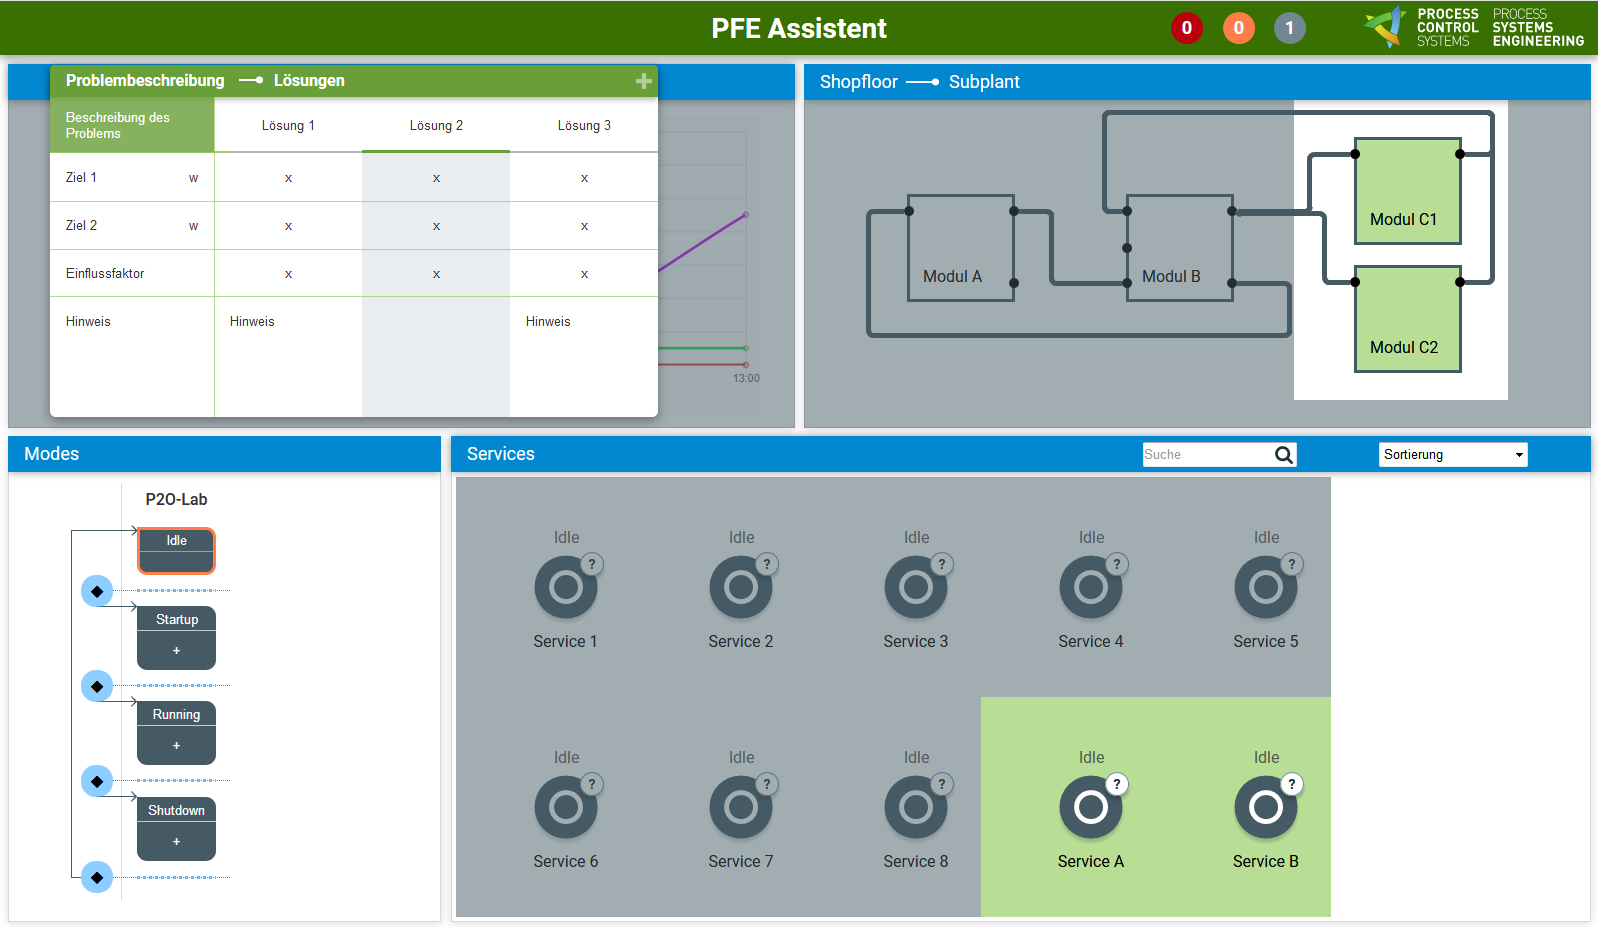
\includegraphics[scale=0.24]{DA_files/Bilder/Konzept/Skizze-Loesungen-PFE.png}
%[keepaspectratio, width=13 cm]
\end{center}
\vspace{2pt}